\documentclass[simplex.tex]{subfiles}
% DO NOT INCLUDE PREAMBLES/PACKAGES HERE!!
% packages are inherited from preamble.tex; you can compile this on its own
\begin{document}
\subsection{CLARITY}

\subsubsection{CLARITY registration Pipeline}

%We are working on migrating our exisiting CLARITY pipeline to run entirely on virtualized infrastructure in the cloud.
%This workflow includes ingesting into ndstore, aligning to a reference atlas, and storing a registered stack back into ndstore.
%Currently, ndstore is working the cloud, with manual ingest of data.
%The next steps are to deploy LDDMM via Docker containers to run within the cloud environment.
We tested our complete registration pipeline on a new CLARITY brain image from our Stanford collaborators.
The image was acquired at a $0.585 \mu m \times 0.585 \mu m \times 5 \mu m$ resolution using light-sheet microscopy.
After sub-volume stitching, the volume was ingested into ndstore and propagated to lower resolutions.
It was then downloaded at the 6th resolution level ($37.44 \mu m \times 37.44 \mu m \times 5 \mu m$) for registration with Allen Reference Atlas (ARA).
The registration pipeline began by aligning the ARA's Scanning Two-Photon (STP) tomography image using a 12-parameter affine model under Mutual Information (MI) matching.
Next deformable registration was then done using MI-based Large Deformation Diffeomorphic Metric Mapping (MI-LDDMM).
CLARITY-aligned annotations were generated by applying the resulting inverse transform to the ARA annotations.
These annotations were uploaded into ndstore for visualization in NeuroDataViz's new Neuroglacer interface.

\begin{figure}[!h]
\begin{cframed}
\centering
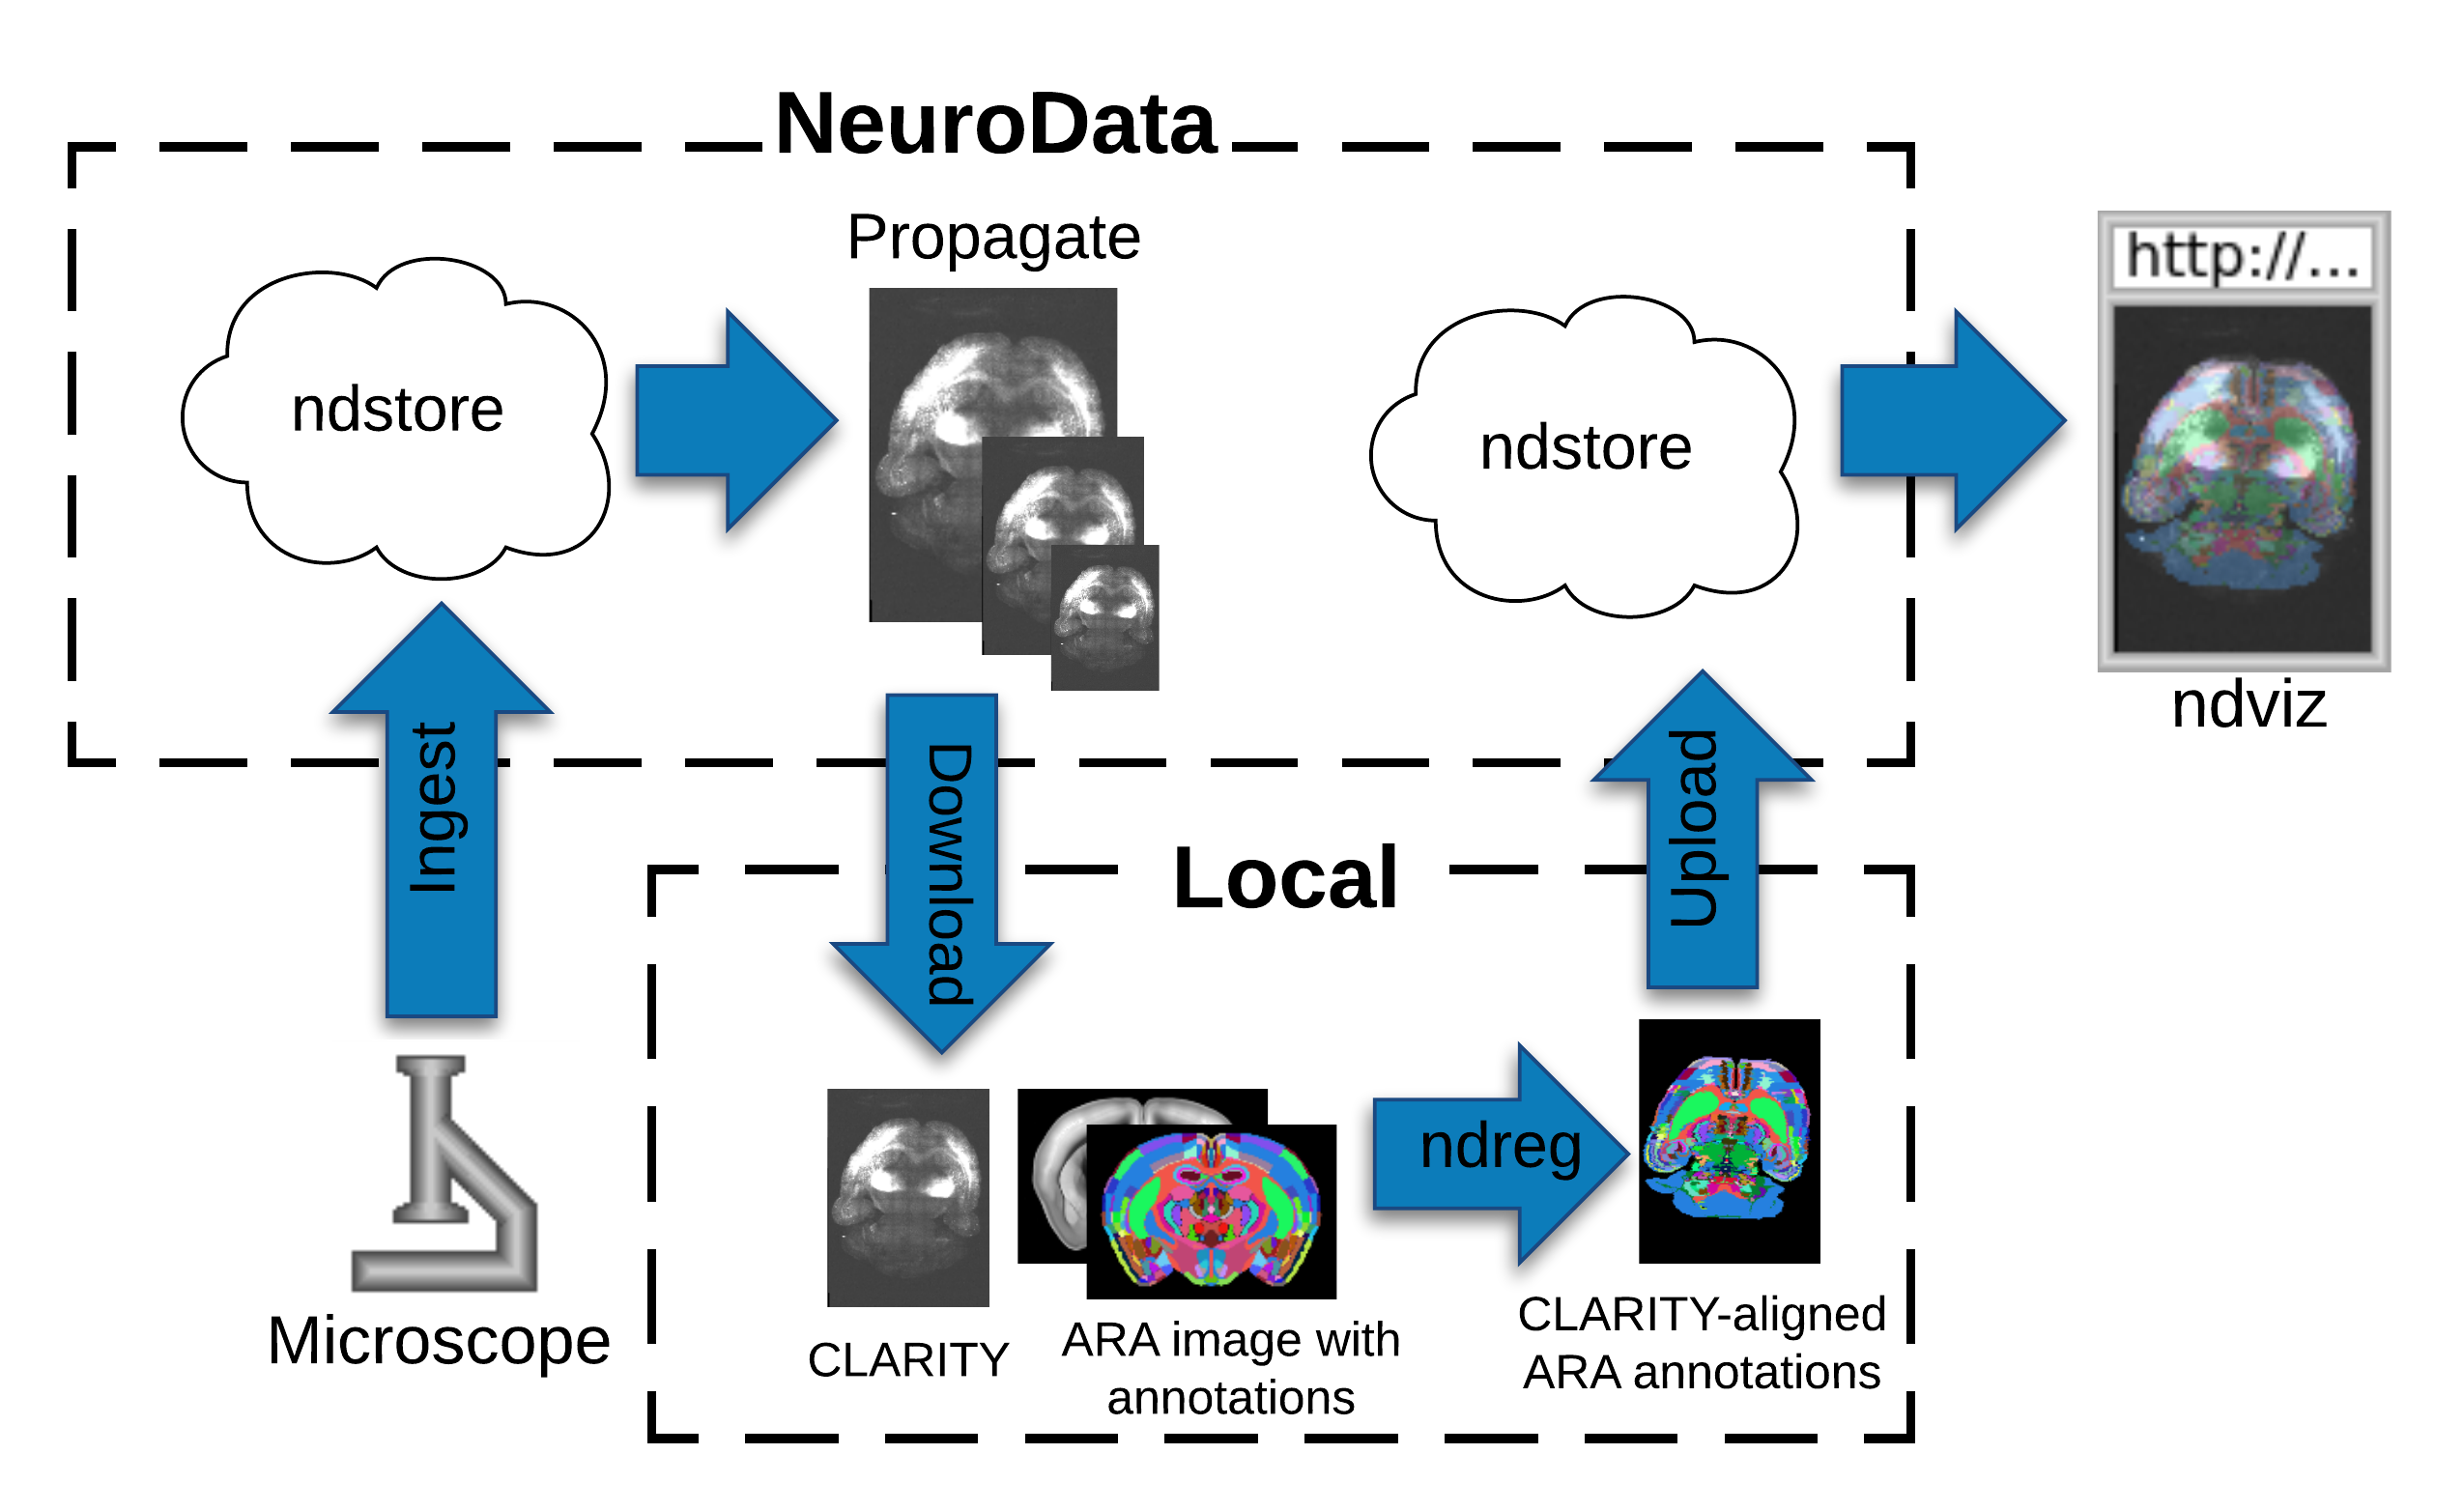
\includegraphics[width=0.95\textwidth]{../../figs/workflow.png}
\caption{Workflow from microscope to visualization in NeuroDataViz (ndviz)}
\label{fig:name}
\end{cframed}
\end{figure}


\end{document}
